\documentclass[hidelinks,12pt]{article}
\usepackage[left=0.25cm,top=1cm,right=0.25cm,bottom=1cm]{geometry}
%\usepackage[landscape]{geometry}
\textwidth = 20cm
\hoffset = -1cm
\usepackage[utf8]{inputenc}
\usepackage[spanish,es-tabla]{babel}
\usepackage[autostyle,spanish=mexican]{csquotes}
\usepackage[tbtags]{amsmath}
\usepackage{nccmath}
\usepackage{amsthm}
\usepackage{amssymb}
\usepackage{mathrsfs}
\usepackage{graphicx}
\usepackage{subfig}
\usepackage{standalone}
\usepackage[outdir=./Imagenes/]{epstopdf}
\usepackage{siunitx}
\usepackage{physics}
\usepackage{color}
\usepackage{float}
\usepackage{hyperref}
\usepackage{multicol}
%\usepackage{milista}
\usepackage{anyfontsize}
\usepackage{anysize}
%\usepackage{enumerate}
\usepackage[shortlabels]{enumitem}
\usepackage{capt-of}
\usepackage{bm}
\usepackage{relsize}
\usepackage{placeins}
\usepackage{empheq}
\usepackage{cancel}
\usepackage{wrapfig}
\usepackage[flushleft]{threeparttable}
\usepackage{makecell}
\usepackage{fancyhdr}
\usepackage{tikz}
\usepackage{bigints}
\usepackage{scalerel}
\usepackage{pgfplots}
\usepackage{pdflscape}
\pgfplotsset{compat=1.16}
\spanishdecimal{.}
\renewcommand{\baselinestretch}{1.5} 
\renewcommand\labelenumii{\theenumi.{\arabic{enumii}})}
\newcommand{\ptilde}[1]{\ensuremath{{#1}^{\prime}}}
\newcommand{\stilde}[1]{\ensuremath{{#1}^{\prime \prime}}}
\newcommand{\ttilde}[1]{\ensuremath{{#1}^{\prime \prime \prime}}}
\newcommand{\ntilde}[2]{\ensuremath{{#1}^{(#2)}}}

\newtheorem{defi}{{\it Definición}}[section]
\newtheorem{teo}{{\it Teorema}}[section]
\newtheorem{ejemplo}{{\it Ejemplo}}[section]
\newtheorem{propiedad}{{\it Propiedad}}[section]
\newtheorem{lema}{{\it Lema}}[section]
\newtheorem{cor}{Corolario}
\newtheorem{ejer}{Ejercicio}[section]

\newlist{milista}{enumerate}{2}
\setlist[milista,1]{label=\arabic*)}
\setlist[milista,2]{label=\arabic{milistai}.\arabic*)}
\newlength{\depthofsumsign}
\setlength{\depthofsumsign}{\depthof{$\sum$}}
\newcommand{\nsum}[1][1.4]{% only for \displaystyle
    \mathop{%
        \raisebox
            {-#1\depthofsumsign+1\depthofsumsign}
            {\scalebox
                {#1}
                {$\displaystyle\sum$}%
            }
    }
}
\def\scaleint#1{\vcenter{\hbox{\scaleto[3ex]{\displaystyle\int}{#1}}}}
\def\bs{\mkern-12mu}


%\usepackage{showframe}
\title{Transformadas de Fourier \\ \large {Tema 6 - Transformadas integrales} \vspace{-3ex}}
\author{M. en C. Gustavo Contreras Mayén}
\date{ }
\begin{document}
\vspace{-4cm}
\maketitle
\fontsize{14}{14}\selectfont
\tableofcontents
\newpage

%Ref. Patra (2018) 1.2 Classes of functions.
\section{Tipos de funciones.}

Una función de valor único $f (x)$ de la variable independiente $x$ que es continua en un intervalo $[a, b]$, se dice que pertenece a una clase denotada por $f \in C \, [a, b]$.
\par
Se dice que una función $f (x)$ es continua por partes en un intervalo $(a, b)$ si el intervalo se puede dividir en un número finito de subintervalos que no se intersectan $(a, a_{1}), (a_{1}, a_{2}), \ldots, (a_{n -1}, b)$, en cada uno de los cuales la función es continua y tiene límites finitos cuando $x$ se acerca a los puntos extremos de cada uno de los subintervalos. Se dice que dicha función pertenece a una clase denotada por $f \in P \, (a, b)$.
\par
Una función continua a trozos $f$ en $(a, b)$, cuya derivada de primer orden es también una función continua a trozos en $(a, b)$ y pertenece a una clase denotada por $f \in P^{1} \, (a, b)$.
\par
Se dice que el conjunto de funciones $f (x)$ es absolutamente integrable sobre $\Omega$, si $\scaleint{6ex}_{\bs \Omega}  \abs{f (x)} \dd{x}$ es finito. Entonces decimos que esta función pertenece a una clase denotada por $f (x) \in A_{1} (\Omega)$. De manera similar, el hecho que $f \in A_{m} (\Omega)$ implica que $\scaleint{6ex}_{\bs \Omega}  \abs{f (x)} \dd{x}$ es finito.
\par
Finalmente, presentamos una clase de funciones $f (x)$, que satisface las siguientes condiciones:
\begin{enumerate}[label=\roman*]
\item $f (x)$ se define en $c < x < c + 2 \, l$.
\item $f (x)$ es una función periódica del período $2 \, l$.
\item $f (x)$ y $\pderivada{f} (x)$ son continuas por partes en $c  < x <c + 2 \, l$ expresado por $f (x) \in P^{1} (c, c + 2 \, l)$.
\end{enumerate}
Se dice que esta clase de función $f (x)$ satisface las condiciones de Dirichlet. Se dice que una función $f (x)$ es de orden exponencial $\sigma$ cuando $x \to \infty$, si las constantes $\sigma, m (> 0)$ se pueden encontrar de modo que:
\begin{align*}
\abs{ e^{\sigma \, x} \, f (x)} < m \hspace{1cm} \Longrightarrow \hspace{1cm} \abs{f (x)} < m \, e^{m \, \sigma} \hspace{0.5cm} x > x_{0}
\end{align*}
De manera equivalente, también se puede escribir $f (x) = 0 \, (e^{m \, \sigma})$ mientras $x \to \infty$.

%Ref. Patra (2018) 1.3 Series de Fourier y la Fórmula Integral de Fourier.

\section{Series de Fourier y la fórmula integral de Fourier.}

Consideremos una función $f (x)$ que satisface las condiciones de Dirichlet en el intervalo $[-l, l]$, la función pertenece a la clase $P^{1} (R)$ y también a la clase $A_{1} (R)$. Sea el período principal de $f (x)$ igual a $2 \, l$. Entonces $f (x)$ admite una representación en una serie de Fourier:
\begin{align*}
f (x) = a_{0} + \nsum_{n=1}^{\infty} \left[ a_{n} \, \cos \left( \dfrac{n \, \pi, \, x}{l}  \right) + b_{n} \, \sin \left( \dfrac{n \, \pi, \, x}{l}  \right) \right]
\end{align*}
donde:
\begin{align*}
a_{0} &= \dfrac{1}{2 \, l} \scaleint{6ex}_{\bs -l}^{l} f (x) \dd{x} \\[0.5em]
(a_{n}, b_{n}) &= \dfrac{1}{l} \scaleint{6ex}_{\bs -l}^{l} f (x) \left[ \cos \left( \dfrac{n \, \pi \, x}{l} \right), \sin \left( \dfrac{n \, \pi \, x}{l} \right) \right] \dd{x}
\end{align*}
entonces:
\begin{align*}
a_{n} - i \, b_{n} = \dfrac{1}{l} \scaleint{6ex}_{\bs -l}^{l} f (x) \, \exp \left( - \dfrac{i \, n \, \pi \, x}{l} \right) \dd{x}
\end{align*}
Definimos a continuación:
\begin{align*}
a_{0} &= c_{0} \\
a_{n} &= c_{n} + c_{-n} \\
i \, b_{n} &= c_{n} - c_{-n}
\end{align*}
Entonces tendremos que:
\begin{align}
\begin{aligned}[b]
f (x) &= c_{0} + \nsum_{n=1}^{\infty} \left[ c_{n} \, \exp \left( -\dfrac{i \, n \, \pi \, x}{l} \right) + c_{-n} \, \exp \left( \dfrac{i \, n \, \pi \, x}{l} \right) \right] = \\[0.5em]
&= \nsum_{-\infty}^{+\infty} c_{n} \, \exp \left( - \dfrac{i \, n \, \pi \, x}{l} \right)
\end{aligned}
\label{eq:ecuacion_01_02}
\end{align}
donde el coeficiente $c_{n}$ es:
\begin{align}
\begin{aligned}[b]
c_{n} &= \dfrac{1}{2 \, l} \scaleint{6ex}_{\bs -l}^{l} f (x) \, \exp \left( \dfrac{i \, n \, \pi, x}{l} \right) \dd{x} = \\[0.5em]
&= \dfrac{1}{2 \, l} \scaleint{6ex}_{\bs -l}^{l} f (t) \, \exp \left( \dfrac{i \, n \, \pi, t}{l} \right) \dd{t}
\end{aligned}
\label{eq:ecuacion_01_03}
\end{align}
Esta es forma de la serie de Fourier se le llama \emph{forma compleja de la serie de Fourier} en el intervalo $(-l , l)$.
\par
Por lo que de las ecs. (\ref{eq:ecuacion_01_02}) y (\ref{eq:ecuacion_01_03}), se obtiene:
\begin{align}
f (x) = \nsum_{-\infty}^{+\infty} \left[ \dfrac{1}{2 \, l} \scaleint{6ex}_{\bs -l}^{l} f (t) \exp \left( \dfrac{i \, n \, \pi \, t}{l} \right) \dd{t} \right] \, \exp \left( - \dfrac{i \, n \, \pi \, x}{l} \right)
\label{eq:ecuacion_01_04}
\end{align}
Ahora hagamos el siguiente cambio de variable:
\begin{align*}
\dfrac{\pi}{l} = \delta \xi
\end{align*}
Notemos que $\delta \xi \to 0$ mientras $l \to \infty$, tal que $l \, \delta \xi = \pi =$ un número finito. Entonces la serie (\ref{eq:ecuacion_01_04}), antes de tomar el límite cuando $\delta \xi \to 0$, se convierte en:
\begin{align*}
f (x) &= \dfrac{1}{2 \, \pi} \nsum_{-\infty}^{+\infty} \delta \xi \, \left[ \scaleint{6ex}_{\bs -\frac{\pi}{\delta \xi}}^{\frac{\pi}{\delta \xi}} f (t) \, \exp \left( i \, n \, t \, \delta \xi \right) \dd{t} \right] \, \exp \left( - i \, n \, x \, \delta \xi \right) = \\[0.5em]
&= \dfrac{1}{2 \, \pi} \scaleint{6ex}_{\bs -\frac{\pi}{\delta \xi}}^{\frac{\pi}{\delta \xi}} f (t) \, \left[ \nsum_{-\infty}^{+\infty} \delta \xi \, \exp \left( i \, n (t - x \, \delta \xi) \right) \right] \dd{t}
\end{align*}
después de intercambiar formalmente los signos de suma e integración. Dado que asumimos que  $f (x) \in P^{1} (R)$ y también que $f (x) \in A_{1} (R)$, haciendo que $\delta \xi \to 0$ y usando la definición de integral definida de Riemann como límite de una suma obtenemos:
\begin{align}
f (x) &= \dfrac{1}{2 \, \pi} \scaleint{6ex}_{\bs -\infty}^{\infty} f (t) \, \left[ \exp \left( i (t - x) \, y \right) \, \dd{y} \right] \dd{t} \label{eq:ecuacion_01_05} \\[0.5em]
\Rightarrow f (x) &= \dfrac{1}{\sqrt{2 \, \pi}} \scaleint{6ex}_{\bs -\infty}^{\infty} \exp \left( i \, y \, x \right) \big[ F (y) \big] \dd{y} \label{eq:ecuacion_01_06} \\[0.5em]
\mbox{donde} \hspace{0.5cm} F (y) &= \dfrac{1}{\sqrt{2 \, \pi}} \scaleint{6ex}_{\bs -\infty}^{\infty} f (t) \, \exp \left( i \, y \, t \right) \dd{t} \label{eq:ecuacion_01_07}
\end{align}
De nueva cuenta, de la ec. (\ref{eq:ecuacion_01_05}), se obtiene lo siguiente:
\begin{align}
f (x) = \dfrac{1}{\pi} \scaleint{6ex}_{\bs 0}^{\infty}  \dd{y} \, \scaleint{6ex}_{\bs -\infty}^{+\infty} f (t) \, \cos y (-t + x) \dd{t} \label{eq:ecuacion_01_08}
\end{align}
La ecuación (\ref{eq:ecuacion_01_08}) se le conoce como la \emph{fórmula integral de Fourier}.
\par
En un punto de discontinuidad finita de $f (x)$, el lado izquierdo de la ec. (\ref{eq:ecuacion_01_08}) se reemplaza con
\begin{align*}
\dfrac{1}{2} \big[ f (x + 0) + f (x - 0) \big]
\end{align*}
en el sentido de los valores límite.

%Referencia. Patra (2018) - An introduction to integral transforms. Sec. 1.4
\section{Las transformadas de Fourier.}

Una vez revisado el material introductorio, podemos definir la \emph{transformada de Fourier} (TF) de una función continua por partes $f (x) \in P^{1} (R)$ y tal que $f (x) \in A_{1} (R)$. La transformada se define por:
\begin{align}
\begin{aligned}[b]
F \big[ f (x); x \to \xi \big] &= F \big[ f (x) \big] = F (\xi) = \overline{f} (\xi) = \\[0.5em] 
&= \dfrac{1}{\sqrt{2 \, \pi}} \scaleint{6ex}_{\bs -\infty}^{+\infty} f (x) \, \exp(i \, \xi \, x) \dd{x}
\end{aligned}
\label{eq:ecuacion_01_12}
\end{align}
y también:
\begin{align}
f (x) = F^{-1} \big[ F (\xi) \big] = \dfrac{1}{\sqrt{2 \, \pi}} \scaleint{6ex}_{\bs -\infty}^{+\infty} F (\xi) \, \exp(-i \, \xi \, x) \dd{\xi}
\label{eq:ecuacion_01_13}
\end{align}
en un punto continuo de $f (x)$.
\par
La función $F (\xi)$ en la ec. (\ref{eq:ecuacion_01_12}) es la \emph{transformada de Fourier} de $f (x)$, mientras que $f (x)$ en la ec. (\ref{eq:ecuacion_01_13}) es la llamada \emph{transformada inversa de Fourier} de $F (\xi)$.
\par
Algunos autores definen la transformada de Fourier  (ec. \ref{eq:ecuacion_01_12}) y la transformada inversa (ec. \ref{eq:ecuacion_01_13}) respectivamente como:
\begin{align}
F \big[ f (x); x \to \xi \big] = F (\xi) = \scaleint{6ex}_{\bs -\infty}^{+\infty} f (x) \, \exp(i \, \xi \, x) \dd{x} \label{eq:ecuacion_01_14} \\[0.5em]
f (x) = \dfrac{1}{2 \, \pi} \scaleint{6ex}_{\bs -\infty}^{+\infty} F (\xi) \, \exp(-i \, \xi \, x) \dd{\xi}
\label{eq:ecuacion_01_15}
\end{align}
En un punto de discontinuidad de $x \in R$, el lado izquierdo de las ecs. (\ref{eq:ecuacion_01_13}) y (\ref{eq:ecuacion_01_15}), toman la forma:
\begin{align*}
\dfrac{1}{2} \big[ f(x + 0) + f(x - 0) \big]
\end{align*}
en lugar de $f (x)$.
\par
De las definiciones de las transformadas de Fourier y de la transformada inversa de Fourier, es posible escribir de la ec. (\ref{eq:ecuacion_01_12}):
\begin{align*}
F (\xi) = F \big[ f (x) \big] = F \big[ F^{1} (F (\xi)) \big] \hspace{0.2cm} &\Rightarrow \hspace{0.2cm} F \, F^{-1} \big[ F (\xi) \big] \equiv I \big[ F (\xi) \big] \\[0.5em]
&\Rightarrow \hspace{0.2cm} F \, F^{-1} = I
\end{align*}
que es un operador de identidad, entonces $F$ y $F^{-1}$ son los operadores de Fourier y su operador inverso respectivamente, y de la ec. (\ref{eq:ecuacion_01_13}):
\begin{align}
\begin{aligned}[b]
f (x) = F^{-1} \big[ F (\xi) \big] = F^{-1} \big[ F(f (x)) \big] &= F^{-1} \, F \big[ f (x) \big] = I \big[ f (x) \big] \\[0.5em]
&\Rightarrow \hspace{0.2cm} F^{-1} \, F = I
\end{aligned}
\label{eq:ecuacion_01_16}
\end{align}
Por lo que en una notación de operador:
\begin{align*}
F \, F^{-1} = F^{-1} \, F = I
\end{align*}
Esto demuestra que los operadores $F$ y $F^{-1}$ son conmutativos.

\subsection{Transformadas seno y coseno de Fourier.}

Consideremos que la función $f (x)$ sea una función \emph{impar} de $x \in R$, perteneciente además a las clases $P^{1} (R)$ y $A_{1} (R)$. Tenemos claramente que $f(-x) = - f (x)$. 
\par
De la ec. (\ref{eq:ecuacion_01_12}):
\begin{align}
\begin{aligned}[b]
F \big[ f (x); x \to \xi \big] = F (\xi) &= \dfrac{1}{\sqrt{2 \, \pi}} \scaleint{6ex}_{\bs 0}^{\infty} f (x) \big[ \exp(i \xi x) {-} \exp(-i \xi x) \big] \dd{x} = \\[0.5em]
&= i \, \sqrt{\dfrac{2}{\pi}} f (x) \, \sin \xi \, x \dd{x} = \\[0.5em]
&\equiv i \, F_{s} (\xi)
\end{aligned}
\label{eq:ecuacion_01_17}
\end{align}
donde:
\begin{align}
F_{s} (\xi) = \sqrt{\dfrac{2}{\pi}} f (x) \, \sin \xi \, x \dd{x}
\label{eq:ecuacion_01_18}
\end{align}
La ec. (\ref{eq:ecuacion_01_18}) define la \emph{transformada seno de Fourier} de la función $f (x)$.
\par
Su conexión con la transformada de Fourier, está dada por la ec. (\ref{eq:ecuacion_01_17}) proporcionando $f (x)$ una función impar de $x \in R$. La expresión para la transformada inversa de (\ref{eq:ecuacion_01_18}) se define por:
\begin{align}
f (x) = \sqrt{\dfrac{2}{\pi}} \scaleint{6ex}_{\bs 0}^{\infty} F_{s}(\xi) \, \sin \xi \, x \dd{\xi}
\label{eq:ecuacion_01_19}
\end{align}
Sea ahora una función par $f (x)$ de $x \in R$, además de que pertenece a la clases $P^{1}(R)$ y $A_{1}(R)$. Entonces: $f(-x) = f (x)$, por lo tanto, por la ec. (\ref{eq:ecuacion_01_12}):
\begin{align}
\begin{aligned}[b]
F \big[ f (x); x \to \xi \big] = F (\xi) &= \dfrac{1}{\sqrt{2 \, \pi}} \scaleint{6ex}_{\bs 0}^{\infty} f (x) \big[ \exp(i \xi x) {+} \exp(-i \xi x) \big] \dd{x} = \\[0.5em]
&= i \, \sqrt{\dfrac{2}{\pi}} f (x) \, \cos \xi \, x \dd{x} = \\[0.5em]
&\equiv i \, F_{c} (\xi)    
\end{aligned}
\label{eq:ecuacion_01_20}
\end{align}
donde:
\begin{align}
F_{c} (\xi) = \sqrt{\dfrac{2}{\pi}} f (x) \, \cos \xi \, x \dd{x}
\label{eq:ecuacion_01_21}
\end{align}
La ec. (\ref{eq:ecuacion_01_21}) define la \emph{transformada coseno de Fourier} de la función $f (x)$.
\par
Su conexión con la transformada de Fourier, está dada por la ec. (\ref{eq:ecuacion_01_20}) proporcionando $f (x)$ una función par de $x \in R$. La expresión para la transformada inversa de (\ref{eq:ecuacion_01_21}) se define por:
\begin{align}
f (x) = \sqrt{\dfrac{2}{\pi}} \scaleint{6ex}_{\bs 0}^{\infty} F_{c}(\xi) \, \cos \xi \, x \dd{\xi}
\label{eq:ecuacion_01_22}
\end{align}

\subsection{Propiedad de linealidad.}

Si $c_{1}$ y $c_{2}$ son constantes, entonces:
\begin{enumerate}[\thesubsection .1)]
\item \label{inciso_01} $F \big[ c_{1} \, f_{1} (x) + c_{2} \, f_{2} (x) \big] = c_{1} \, F \big[ f_{1} (x) \big] + c_{2} \, F \big[ f_{2} (x) \big]$
\item $F_{s} \big[ c_{1} \, f_{1} (x) + c_{2} \, f_{2} (x) \big] = c_{1} \, F_{s} \big[ f_{1} (x) \big] + c_{2} \, F_{s} \big[ f_{2} (x) \big]$
\item $F_{c} \big[ c_{1} \, f_{1} (x) + c_{2} \, f_{2} (x) \big] = c_{1} \, F_{c} \big[ f_{1} (x) \big] + c_{2} \, F_{c} \big[ f_{2} (x) \big]$
\end{enumerate}
La demostración se sigue de la definición de la transformada de Fourier de la ec. (\ref{eq:ecuacion_01_12}), en el caso del inciso (\ref{inciso_01}, se tiene que: 
\begin{align*}
&F \big[ c_{1} \, f_{1} (x) + c_{2} \, f_{2} (x) ; x \to \xi \big] = \\[0.5em]
&= \dfrac{1}{\sqrt{2 \, \pi}} \scaleint{6ex}_{\bs -\infty}^{\infty} \big[ c_{1} \, f_{1} (x) + c_{2} \, f_{2} (x) \big] \, \exp(i \xi x) \dd{x} = \\[0.5em]
&= c_{1} \, \dfrac{1}{\sqrt{2 \, \pi}} \scaleint{6ex}_{\bs -\infty}^{\infty} f_{1}(x) \, \exp(i \xi x) \dd{x} + c_{2} \, \dfrac{1}{\sqrt{2 \, \pi}} \scaleint{6ex}_{\bs -\infty}^{\infty} f_{2}(x) \, \exp(i \xi x) \dd{x} = \\[0.5em]
&= c_{1} \, F \big[ f_{1} (x) ; x \to \xi \big] + c_{2} \, F \big[ f_{2} (x) ; x \to \xi \big]
\end{align*}
La demostración de los otros dos incisos es análoga.

\subsection{Propiedad de cambio de escala.}

\begin{enumerate}[\thesubsection .1)]
\item Si $F \big[ f (x); x \to \xi \big] = F (\xi)$, entonces
\begin{align*}
F \big[ f(a \, x); x \to \xi \big] = \dfrac{1}{a} \, F \left( \dfrac{\xi}{a} \right)
\end{align*}
\item \label{inciso_01_06_01} Si $F_{s} \big[ f (x) \big] = F_{s}(\xi)$, entonces
\begin{align*}
F_{s} \big[f(a \, x) \big] = \dfrac{1}{a} \, F_{s} \left( \dfrac{\xi}{a} \right)
\end{align*}
\item Si $F_{c} \big[ f (x); x \to \xi \big] = F_{c}(\xi)$, entonces
\begin{align*}
F_{c} \big[ f(a \, x); x \to \xi \big] = \dfrac{1}{a} \, F_{c} \left( \dfrac{\xi}{a} \right)
\end{align*}
\end{enumerate}
La demostración del inciso (\ref{inciso_01_06_01} se sigue de la definición:
\begin{align*}
F_{s} \big[ f (x); x \to \xi \big] = \sqrt{\dfrac{2}{\pi}} \scaleint{6ex}_{\bs 0}^{\infty} f (x) \, \sin \xi \, x \dd{\xi} = F_{s} (\xi)
\end{align*}
por lo que:
\begin{align*}
&F_{s} \big[ f(a \, x); x \to \xi \big] = \sqrt{\dfrac{2}{\pi}} \scaleint{6ex}_{\bs 0}^{\infty} f(a \, x) \, \sin \xi \, x \dd{\xi} = \\[0.5em]
&= \dfrac{1}{a} \, \sqrt{\dfrac{2}{\pi}} \scaleint{6ex}_{\bs 0}^{\infty} f(t) \sin \left( \dfrac{\xi}{a} \, t \right) \dd{t} = \\[0.5em]
&= \dfrac{1}{a} \, F_{s} \left( \dfrac{\xi}{a} \right)
\end{align*}
La demostración de los otros dos incisos, se sigue de la misma manera, ocupando la definición de la transformada de Fourier y la transformada coseno de Fourier.

\subsection{Propiedad de desplazamiento.}

Si $F (\xi)$ es la transformada de Fourier de $f (x)$ en $R$, entonces la transformada de Fourier de $f(x - a)$ es:
\begin{align*}
f(x - a) = \exp(i \, \xi \, a) \, F (\xi)
\end{align*}
Comenzamos la demostración de la propiedad de desplazamiento a partir de la definición:
\begin{align*}
F (\xi) = \dfrac{1}{\sqrt{2 \, \pi}} \scaleint{6ex}_{\bs -\infty}^{+\infty} f (x) \, \exp(i \, \xi \, x) \dd{x} = F \big[ f (x); x \to \xi \big]
\end{align*}
Por lo tanto:
\begin{align*}
F \big[ f(x - a); x \to \xi \big] &= \dfrac{1}{\sqrt{2 \, \pi}} \scaleint{6ex}_{\bs -\infty}^{+\infty} f(x - a) \, \exp(i \, \xi \, x) \dd{x} \\[0.5em]
&= \dfrac{1}{\sqrt{2 \, \pi}} \scaleint{6ex}_{\bs -\infty}^{+\infty} f(t) \, \exp(i \, \xi (t + a)) \dd{t} \\[0.5em]
&= \exp(i \, \xi \, a) \, \dfrac{1}{\sqrt{2 \, \pi}} \scaleint{6ex}_{\bs -\infty}^{+\infty} f(t) \, \exp(i \, \xi \, t) \dd{t} \\[0.5em]
&= \exp(i \, \xi \, a) \, F (\xi) 
\end{align*}

\subsection{El teorema de modulación.}

\textbf{Teorema:} Si $F \big[ f (x); x \to \xi \big] = F (\xi)$, entonces:
\begin{align*}
F \big[ f (x) \, \cos a \, x; x \to \xi \big] = \dfrac{1}{2} \big[F(\xi + a) + F(\xi - a) \big]
\end{align*}
\textbf{Demostración:}
\\
Ya que se tiene:
\begin{align*}
F \big[f (x); x \to \xi \big] = F (\xi) = \dfrac{1}{\sqrt{2 \, \pi}} \scaleint{6ex}_{\bs -\infty}^{+\infty} f (x) \, \exp(i \, \xi \, x) \dd{x}
\end{align*}
entonces:
\begin{align*}
F \big[ f (x); x \to \xi \big] &= \dfrac{1}{\sqrt{2 \, \pi}} \scaleint{6ex}_{\bs -\infty}^{+\infty} f (x) \, \dfrac{\exp(i \, a \, x) + \exp(-i \, a \, x)}{2} \, \exp(i \, \xi \, x) \dd{x} = \\[0.5em]
&= \dfrac{1}{2} \left[ \dfrac{1}{\sqrt{2 \, \pi}} \scaleint{6ex}_{\bs -\infty}^{+\infty} f (x) \, \exp(i \, (\xi + a) \, x)  \dd{x} + \right. \\[0.5em]
&+ \left. \dfrac{1}{\sqrt{2 \, \pi}} \scaleint{6ex}_{\bs -\infty}^{+\infty} f (x) \, \exp(i \, (\xi - a) \, x)  \dd{x} \right] = \\[0.5em]
&= \big[ F(\xi + a) + F (\xi - a) \big]
\end{align*}
Otras tres partes del teorema son:
\begin{enumerate}[label=\alph*)]
\item Si $F_{s} \big[ f (x); x \to \xi \big] = F_{s} (\xi)$, entonces
\begin{align*}
F_{s} \big[ f (x) \, \cos a \, x; x \to \xi \big] = \dfrac{1}{2} \big[ F_{s} (\xi +  a) + F_{s} (\xi - a) \big]
\end{align*}
\item Si $F_{s} \big[ f (x); x \to \xi \big] = F_{s} (\xi)$, entonces
\begin{align*}
F_{c} \big[ f (x) \, \sin a \, x; x \to \xi \big] = \dfrac{1}{2} \big[ F_{s} (\xi +  a) - F_{s} (\xi - a) \big]
\end{align*}
\item Si $F_{c} \big[f (x); x \to \xi \big] = F_{c} (\xi)$, entonces
\begin{align*}
F_{s} \big[f (x) \, \sin a \, x; x \to \xi \big] = \dfrac{1}{2} \big[ F_{c} (\xi -  a) - F_{c} (\xi + a) \big]
\end{align*}
\end{enumerate}
Estos resultados pueden demostrarse de manera similar como se hizo en el primer caso al reemplazar $\cos a \, x$ y $\sin a \, x$ por sus formas exponenciales en las definiciones de las transformadas correspondientes del lado izquierdo.

\subsection{Evaluación de integrales mediante transformadas inversas.}

Por definiciones de la transformada de Fourier y su transformada inversa en las ecs. (\ref{eq:ecuacion_01_12}), (\ref{eq:ecuacion_01_13}), (\ref{eq:ecuacion_01_17}), (\ref{eq:ecuacion_01_19}), (\ref{eq:ecuacion_01_21}) y (\ref{eq:ecuacion_01_22}), podemos emplear esos resultados para evaluar ciertas integrales que involucran funciones trigonométricas. 
\bigskip

\noindent
\textbf{Ejemplo 1.}
\\
En primer lugar consideramos:
\begin{align*}
I_{1} = \scaleint{6ex}_{\bs 0}^{\infty} \exp (-b \, x) \, \cos a \, x \dd{x}, \hspace{1cm} I_{2} = \scaleint{6ex}_{\bs 0}^{\infty} \exp (-b \, x) \, \sin a \, x \dd{x}
\end{align*}
Integrando por partes podemos evaluar $I_{1}$ e $I_{2}$ como
\begin{align*}
I_{1} = \dfrac{b}{a^{2} + b^{2}},  \hspace{1.5cm} I_{2} = \dfrac{a}{a^{2} + b^{2}}
\end{align*}
Estos resultados implican que si hacemos $f (x) = \exp(-b \, x)$, entonces las transformadas seno y coseno están dadas por:
\begin{align*}
F_{c} \big[ \exp(-b \, x); x \to \xi \big] &= \sqrt{\dfrac{2}{\pi}} \, \dfrac{b}{\xi^{2} + b^{2}} \\[0.5em]
F_{s} \big[ \exp(-b \, x); x \to \xi \big] &= \sqrt{\dfrac{2}{\pi}} \, \dfrac{\xi}{\xi^{2} + b^{2}}
\end{align*}
Al sustituir éstas expresiones en las ecs. (\ref{eq:ecuacion_01_19}) y (\ref{eq:ecuacion_01_22}), tenemos que:
\begin{align*}
\scaleint{6ex}_{\bs 0}^{\infty} \dfrac{\cos \xi \, x}{\xi^{2} + b^{2}} \dd{\xi} &= \dfrac{\pi}{2 \, b} \, \exp(-b \, x) \\[1em]
\scaleint{6ex}_{\bs 0}^{\infty} \dfrac{\xi \, \sin \xi \, x}{\xi^{2} + b^{2}} \dd{\xi} &= \dfrac{\pi}{2} \, \exp(-b \, x)
\end{align*}
\bigskip

\noindent
\textbf{Ejemplo 2.}
\\
Si hacemos que la función $f (x)$ sea tal que:
\begin{align*}
f (x) = \begin{cases}
1, & 0 < x < a \\[0.5em]
0, & x > a
\end{cases}
\end{align*}
entonces
\begin{align*}
F_{c}(\xi) = \dfrac{2}{\pi} \scaleint{6ex}_{\bs 0}^{a} 1 \, \cos \xi \, x \dd{x} = \sqrt{\dfrac{2}{\pi}} \, \dfrac{\sin \xi \, a}{\xi}
\end{align*}
para así obtener:
\begin{align*}
\dfrac{2}{\pi} \scaleint{6ex}_{\bs 0}^{a} \, \dfrac{\sin \xi \, a}{\xi} \, \cos \xi \, x \dd{x} = \begin{cases}
1, & \mbox{si } 0 < x < a \\[0.5em]
0, & \mbox{si } x \geq a
\end{cases}
\end{align*}

\subsection{Transformada de Fourier de algunas funciones particulares.}

Consideremos la siguiente función \enquote{escalón} $f (x)$, definida por:
\begin{align*}
f (x) = \begin{cases}
0, & x < 0 \\[0.5em]
1, & x > 0
\end{cases}
\end{align*}
Esta función se conoce como la \emph{función de paso unitario de \textbf{Heaviside}}, que se representa como $H (x)$ y se muestra en la figura (\ref{fig:figura_plot_Heaviside}). Entonces se tiene que:
\begin{align*}
H (x) = \begin{cases}
0, & x < 0 \hspace{0.3cm} (\mbox{o también para } x \leq 0 ) \\[0.5em]
1, & x > 0
\end{cases}
\end{align*}
\begin{figure}[H]
    \centering
    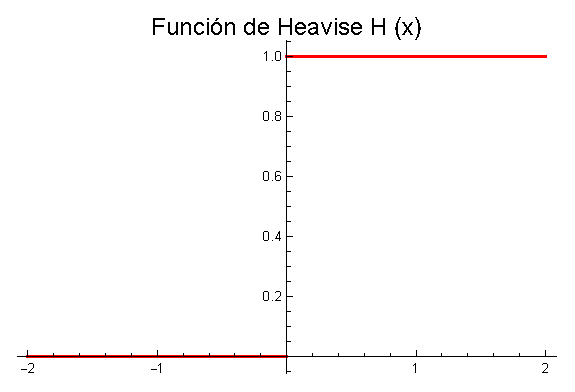
\includegraphics[scale=1]{Imagenes/Plot_Heaviside.eps}
    \caption{Función de Heaviside.}
    \label{fig:figura_plot_Heaviside}
\end{figure}
Casi todas las funciones escalonadas se pueden expresar como una combinación de funciones escalonadas unitarias de Heaviside. Por ejemplo:
\begin{align*}
f (x) = \begin{cases}
1, & \abs{x} < a \\[0.5em]
0, & \mbox{de otra manera}
\end{cases}
\end{align*}
es equivalente a:
\begin{align*}
f (x) = H (x + a) - H (x- a) \equiv H (a - \abs{x})
\end{align*}
La función escalón:
\begin{align*}
f (x) = \begin{cases}
k, & x > a \\[0.5em]
0, & \mbox{de otra manera}
\end{cases}
\end{align*}
es equivalente a:
\begin{align*}
f (x) = k \, H (x - a) \hspace{0.3cm} \forall \, x
\end{align*}
\bigskip

\noindent
\textbf{Ejemplo 3.}
\\
Evaluar la transformada de Fourier de:
\begin{align*}
H (x + a) - H (x - a)
\end{align*}

Por definición:
\begin{align*}
&F \big[ H(x + a) - H(x - a); x \to \xi \big] = \\[0.5em]
&= \dfrac{1}{\sqrt{2\, \pi}} \scaleint{6ex}_{\bs 0}^{\infty} \exp(i \, \xi \, x) \big[ H (x + a) - H (x - a) \big] \dd{x} = \\[0.5em]
&= \dfrac{1}{\sqrt{2\, \pi}} \scaleint{6ex}_{\bs -a}^{a} \exp(i \, \xi \, x) \dd{x} = \\[0.5em]
&= \dfrac{1}{\sqrt{2\, \pi}} \, \left[ \dfrac{\exp(i \, \xi \, x)}{i \, \xi} \right] \eval_{-a}^{a} = \\[0.5em]
&= \dfrac{1}{\sqrt{2\, \pi} \, i \, \xi} \, \big[ \exp(i \, \xi \, a) - \exp(-i \, \xi \, ) \big] = \\[0.5em]
&= \sqrt{\dfrac{2}{\pi}} \dfrac{\sin a \, \xi}{\xi}
\end{align*}
Por lo que, usando la transformada de Fourier inversa, se obtiene:
\begin{align*}
\dfrac{1}{\sqrt{2 \, \pi}} \, \scaleint{6ex}_{\bs -\infty}^{+\infty} \sqrt{\dfrac{2}{\pi}} \, \dfrac{\sin a \, \xi}{\xi} \, \exp(- i \, \xi \, x) \dd{\xi}  = H(x + a) - H(x- a)
\end{align*}
Este resultado implica que:
\begin{align*}
\dfrac{1}{\pi} \scaleint{6ex}_{\bs -\infty}^{+\infty} \dfrac{\sin a \, \xi}{\xi} \, \big[ \cos \xi \, x - i \, \sin \xi \, x \big] \dd{x} = H(x + a) - H(x - a)
\end{align*}
es decir:
\begin{align*}
\scaleint{6ex}_{\bs -\infty}^{+\infty} \dfrac{\sin a \, \xi}{\xi} \, \cos \xi \, x \dd{x} &= \pi \, \big[ H(x + a) - H(x - a) \big]  = \\[0.5em]
&= \begin{cases}
\pi, & \mbox{para  } \abs{x} < a \\[0.5em]
0, & \mbox{para  } \abs{x} > a
\end{cases}
\end{align*}
Haciendo que $x = 0$ y $a = 1$, en la expresión anterior tenemos que:
\begin{align*}
\scaleint{6ex}_{\bs -\infty}^{+\infty} \dfrac{\sin a \, \xi}{\xi} = \pi
\end{align*}
lo que implica que:
\begin{align*}
\scaleint{6ex}_{\bs 0}^{\infty} \dfrac{\sin a \, \xi}{\xi} = \dfrac{\pi}{2}
\end{align*}
y además
\begin{align*}
\scaleint{6ex}_{\bs -\infty}^{+\infty} \dfrac{\sin a \, \xi \, \sin \xi \, x}{\xi} = 0
\end{align*}

\noindent
\textbf{Ejemplo 4.}
\\
Evalúa la transformada de Fourier de la función definida\footnote{Considera que el graficador \enquote{une} con la línea la parte en donde se presenta la discontinuidad, dando la impresión de que la gráfica mantiene una continuidad en el trazo.} (ver fig. \ref{fig:figura_plot_Ejemplo_04_01}):
\begin{align*}
f (x) = \begin{cases}
x, & \abs{x} < a \\
0, & \abs{x} > a
\end{cases}
\end{align*}
\begin{figure}[H]
    \centering
    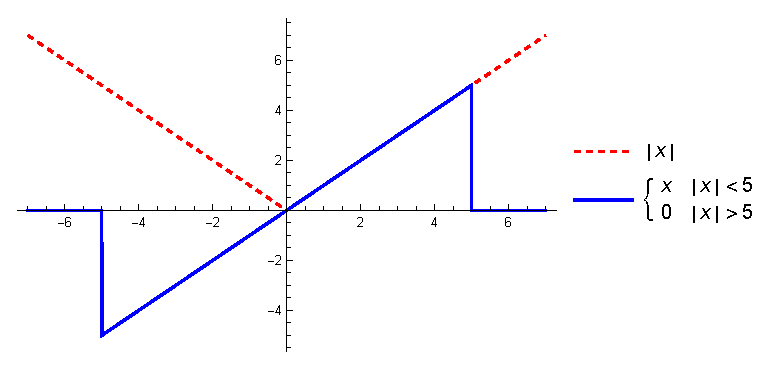
\includegraphics[scale=1]{Imagenes/Plot_Ejemplo_04_01.eps}
    \caption{Función en partes para el Ejemplo 4.}
    \label{fig:figura_plot_Ejemplo_04_01}
\end{figure}

Por definición:
\begin{align*}
F \big[ f (x); x \to \xi \big] &= \dfrac{1}{\sqrt{2 \pi}} \scaleint{6ex}_{\bs -a}^{a} x \, \exp(i \xi x) \dd{x} = \\[0.5em]
&= \dfrac{1}{\sqrt{2 \pi}} \left\{ \bigg[ x \, \dfrac{\exp(i \xi x)}{i \xi} \bigg] \eval_{-a}^{a} - \dfrac{1}{i \xi} \scaleint{6ex}_{\bs -a}^{a} \exp(i \xi x) \dd{x} \right\} = \\[0,5em]
&= \dfrac{1}{\sqrt{2 \pi}} \bigg[ \dfrac{a \exp(i \xi a) + a \exp(-i \xi a)}{i \xi} {+} \\[0.5em]
&+ \dfrac{1}{\xi^{2}} \left\{ \exp(i a \xi) {-} \exp(-i a \xi) \right\} \bigg] = \\[0.5em]
&= \dfrac{1}{\sqrt{2 \pi}} \bigg[ \dfrac{2 \, a \, \cos a \xi}{i \, \xi} + \dfrac{2 \, i \, \sin a \xi}{\xi^{2}} \bigg] = \\[0.5em]
&= \sqrt{\dfrac{2}{\pi}} \, i \, \bigg[ \dfrac{\sin a \, \xi - a \, \xi \, \cos a \xi}{\xi^{2}} \bigg]
\end{align*}
En la figura (\ref{fig:figura_plot_Ejemplo_04_02}) se muestra la gráfica de la Transformada de Fourier $F (\xi)$, el factor $i$ imaginario establece que la transformada esté en el plano complejo.
\begin{figure}[H]
    \centering
    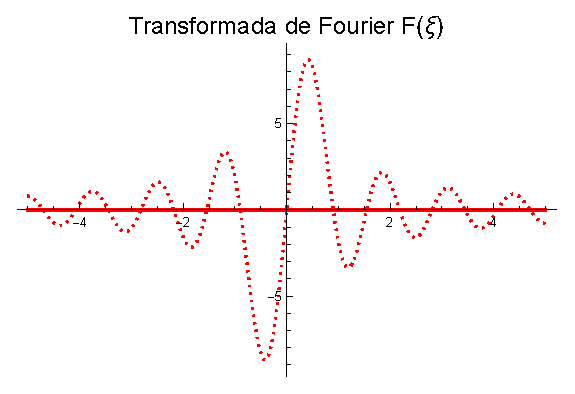
\includegraphics[scale=1]{Imagenes/Plot_Ejemplo_04_02.eps}
    \caption{La transformada de Fourier $F (\xi)$, se muestra la parte imaginaria.}
    \label{fig:figura_plot_Ejemplo_04_02}
\end{figure}
\noindent
\textbf{Ejemplo 5.}
\\
Si la transformada de Fourier de $f (x)$ es $F (\xi)$, calcula la transformada de Fourier en términos de $F (\xi)$:
\begin{enumerate}[label=\roman*)]
\item $\exp(i \lambda x) \, f (x)$
\item $f(-x)$
\end{enumerate}

Sabemos que:
\begin{align*}
F \big[ f (x); x \to \xi \big] = \dfrac{1}{\sqrt{2 \pi}} \scaleint{6ex}_{-\infty}^{+\infty} f (x) \, \exp(i \xi x) \dd{x} = F (\xi)
\end{align*}
Por lo tanto:
\begin{enumerate}[label=(\roman*)]
\item \begin{flalign*}
F \big[ \exp(i \lambda x) \, f (x); x \to \xi \big] &= \dfrac{1}{\sqrt{2 \pi}} \scaleint{6ex}_{-\infty}^{+\infty} f (x) \cdot \exp(i (\xi + \lambda) x) \dd{x} = \\[0.5em]
&= F(\xi + \lambda)
\end{flalign*}
\item \begin{flalign*}
F \big[ f(-x); x \to \xi \big] &= \dfrac{1}{\sqrt{2 \pi}} \scaleint{6ex}_{-\infty}^{+\infty} f(-x) \, \exp(i (\xi + \lambda) x) \dd{x} = \\[0.5em]
&= \dfrac{1}{\sqrt{2 \pi}} \scaleint{6ex}_{-\infty}^{+\infty} f(y) \, \exp(-i \xi y) \dd{y} = \\[0.5em]
&= F^{-1} (\xi)
\end{flalign*}
\end{enumerate}

\subsection{Convolución de dos funciones integrables.}

La convolución\footnote{El término convolución no aparece en el diccionario de la Real Academia Española; su empleo matemático es una castellanización del término inglés \enquote{Convolution} (twist together) cuyo significado más idóneo es: \enquote{retorcido conjunto}. En alemán es \enquote{faltung} (doblar), y en francés, \enquote{composition}.} de dos funciones integrables $f (x)$ y $g(x)$, donde \hfill \break
$-\infty < x < \infty$ se escribe y se define como:
\begin{align}
f * g = \dfrac{1}{\sqrt{2 \, \pi}} \scaleint{6ex}_{\bs -\infty}^{+\infty} f(x - u) \, g(u) \dd{u}
\label{eq:ecuacion_01_23}
\end{align}
La convolución tiene varias propiedades como:
\begin{align*}
f * (\lambda \, g) &= (\lambda \, f) * g = \lambda (f * g), \hspace{1cm} \lambda = \mbox{constante} \\[0.5em]
f * g &= g * f \hspace{1.5cm} \mbox{propiedad conmutativa} \\[0.5em]
f * (g + h) &= f * g + f * h
\end{align*}
que se puede verificar fácilmente directamente desde la definición (\ref{eq:ecuacion_01_23}). \hfill \break 
Además, si tanto $f (x)$ como $g (x)$ pertenecen a las clases $C^{1} (R)$ y $A_{1} (R)$, entonces también lo hace su convolución $h (x) = f * g$, ya que:
\begin{align*}
\sqrt{2 \, \pi} \, \scaleint{6ex}_{\bs -\infty}^{+\infty} \abs{h(x)} \dd{x} &= \scaleint{6ex}_{\bs -\infty}^{+\infty} \dd{x} \, \abs{\scaleint{6ex}_{\bs -\infty}^{+\infty} f(u) g(x - u) \dd{u}} < \\[0.5em]
&< \scaleint{6ex}_{\bs -\infty}^{+\infty} \dd{x} \, \scaleint{6ex}_{\bs -\infty}^{+\infty} \abs{f(u) g(x - u)} \dd{u} = \\[0.5em]
&= \scaleint{6ex}_{\bs -\infty}^{+\infty} \abs{f(u)} \dd{u} \, \scaleint{6ex}_{\bs -\infty}^{+\infty} \abs{g(x - u)} \dd{u} \\[0.5em]
\Rightarrow \scaleint{6ex}_{\bs -\infty}^{+\infty} \abs{h(x)} \dd{x} &< \dfrac{1}{\sqrt{2 \, \pi}} \scaleint{6ex}_{\bs -\infty}^{+\infty} \abs{f(u)} \dd{u} \, \scaleint{6ex}_{\bs -\infty}^{+\infty} \abs{g(\nu)} \dd{\nu}
\end{align*}
y el resultado se sigue del hecho que tanto $f (x)$ y $g(x)$ perteneces a la clase $A_{1}(R)$.
\par
Nuevamente $(f * g) * h = f * (g * h)$ es cierto haciendo una revisión directa. Por lo tanto la propiedad de convolución es también asociativa.
\par
Ahora discutiremos la transformada de Fourier de la convolución de un par de funciones, con el nombre de convolución o teorema de Faltung o Faltung para la Transformada de Fourier.

\subsection{Teorema de convolución para la Transformada de Fourier.}

\textbf{Teorema.}

La transformada de Fourier de $f (x)$ y $g(x)$, ambas funciones pertenecen a las clases $C^{1}(R)$ y $A_{1}(R)$, es el producto de las transformadas de Fourier de $f (x)$ y $g(x)$. Es decir:
\begin{align*}
F \big[f * g; x \to \xi \big] &= F (\xi) \, G(\xi) \\[0.5em]
\mbox{donde } \hspace{0.4cm} F (\xi) &= \dfrac{1}{\sqrt{2 \, \pi}} \scaleint{6ex}_{\bs -\infty}^{\infty} f (x) \, \exp(i \, \xi, x) \dd{x} \hspace{0.3cm} \mbox{y} \\[0.5em]
G(\xi) &= \dfrac{1}{\sqrt{2 \, \pi}} \scaleint{6ex}_{\bs -\infty}^{\infty} g(x) \, \exp(i \, \xi, x) \dd{x}
\end{align*}
\textbf{Demostración: }

Ya que tanto $f (x)$ como $g(x)$ pertenecen ambas a las clases $C^{1}(R)$ y $A_{1}(R)$, se tiene que $f * g$ también pertenece a las clases $C^{1}(R)$ y $A_{1}(R)$, por lo que la transformada de Fourier de $f * g$ también existe. Por lo que:
\begin{align}
\hspace*{-0.5cm}
\begin{aligned}[b]
F \big[f * g; x {\to} \xi \big] &= \dfrac{1}{\sqrt{2 \pi}} \scaleint{6ex}_{\bs -\infty}^{\infty} \! e^{i  \xi x} \dfrac{\dd{x}}{\sqrt{2 \pi}} \scaleint{6ex}_{\bs -\infty}^{\infty} \! f(x {-} u) g(u) \dd{u} \\[0.5em]
&= \dfrac{1}{2 \pi} \scaleint{6ex}_{\bs -\infty}^{\infty} \scaleint{6ex}_{\bs -\infty}^{\infty} \! f(x {-} u) g(u) \exp(i \xi x) \dd{x} \dd{u} = \\[0.5em]
&= \dfrac{1}{2 \pi} \scaleint{6ex}_{\bs -\infty}^{\infty} g(u) \left[ \scaleint{6ex}_{\bs -\infty}^{\infty} \! \exp(i \xi x) f(x {-} u) \dd{x} \right] \dd{u} = \\[0.5em]
&= \dfrac{1}{\sqrt{2  \pi}} \scaleint{6ex}_{\bs -\infty}^{\infty} \! g(u) \exp(i \xi u) \left[ \scaleint{6ex}_{\bs -\infty}^{\infty} \! \exp(i \xi \nu) f(\nu) \dd{\nu} \right] \dd{u} = \\[0.5em]
&= \dfrac{1}{\sqrt{2 \pi}} \scaleint{6ex}_{\bs -\infty}^{\infty} \! g(u) \exp(i  \xi u) \cdot F (\xi) \dd{u} \\[1em]
F \big[f * g; x \to \xi \big] &= F (\xi) \, G(\xi)
\end{aligned}
\label{eq:ecuacion_01_24}
\end{align}
Lo que demuestra el teorema.
\\
\bigskip

\textbf{Corolario 1.}

Otra interpretación del teorema de convolución de la ec. (\ref{eq:ecuacion_01_24}) es tal que:
\begin{align}
\begin{aligned}[b]
&F^{-1} \, \big[F (\xi) \, G(\xi); \xi \to x\big] = \dfrac{1}{\sqrt{2 \, \pi}} \scaleint{6ex}_{\bs -\infty}^{+\infty} f(x - u) \, g(u) \dd{u} \\[0.5em]
&\mbox{O}, \hspace{0.4cm} \dfrac{1}{\sqrt{2 \, \pi}} \scaleint{6ex}_{\bs -\infty}^{+\infty} F (\xi) \, G(\xi) \, \exp(- i \xi x) \dd{\xi} = \dfrac{1}{\sqrt{2 \pi}} \scaleint{6ex}_{\bs -\infty}^{+\infty} f(\nu) g(x - \nu) \dd{\nu} \\[0.5em]
&= f * g
\end{aligned}
\label{eq:ecuacion_01_25}
\end{align}

\textbf{Corolario 2.}

Del resultado anterior (\ref{eq:ecuacion_01_25}), se tiene que:
\begin{align*}
\dfrac{1}{\sqrt{2 \, \pi}} \scaleint{6ex}_{\bs -\infty}^{+\infty} F (\xi) \, G(\xi) \, \exp(- i \xi x) \dd{\xi} &= f * g \\[0.5em]
&= \dfrac{1}{\sqrt{2 \, \pi}} \scaleint{6ex}_{\bs -\infty}^{+\infty} f(\nu) g(x - \nu) \dd{\nu}
\end{align*}
Haciendo que $x = 0$ en la ecuación anterior, vemos que:
\begin{align}
\scaleint{6ex}_{\bs -\infty}^{+\infty} F (\xi) \, G(\xi) \dd{\xi} = \scaleint{6ex}_{\bs -\infty}^{+\infty} f(\nu) g(-\nu) \dd{\nu}
\label{eq:ecuacion_01_26}
\end{align}
\\
\bigskip

\textbf{Corolario 3.}

Sea $f (x) \in R$. Entonces $F (\xi) = F \big[f (x); x \to \xi\big]$ es una función compleja y su conjugado, escrito como $\overline{F}(\xi)$ está dado por:
\begin{align}
\begin{aligned}[b]
\overline{F}(\xi) = \dfrac{1}{\sqrt{2 \, \pi}} \scaleint{6ex}_{\bs -\infty}^{\infty} f (x) \, \exp(-i \, \xi \, x) \dd{x} &= F^{-1} \, \big[f (x); x \to \xi\big] \\[0.5em]
\mbox{es decir} \hspace{0.5cm} \overline{F} \left\{f (x); x \to \xi \right\} &= F^{-1} F^{-1} \, \big[f (x); x \to \xi \big] \\[0.5em]
\mbox{por lo tanto} \hspace{0.5cm} \overline{F} &\equiv F^{-1}
\end{aligned}
\label{eq:ecuacion_01_27}
\end{align}
\\
\bigskip

\textbf{Corolario 4.}

También se pueden establecer resultados similares para las transformadas de seno y coseno de las funciones $f (x)$ y $g (x) \in R$ con respecto a su convolución. Por ejemplo, si $f (x)$, $g (x)$ son funciones pares y
\begin{align}
\begin{aligned}[b]
F_{c} \big[f (x); x \to \xi \big] &= \sqrt{\dfrac{2}{\pi}} \scaleint{6ex}_{\bs 0}^{\infty} f (x) \, \cos \xi \, x \dd{x} \\[0.5em]
F_{c} \big[g(x); x \to \xi \big] &= \sqrt{\dfrac{2}{\pi}} \scaleint{6ex}_{\bs 0}^{\infty} g(x) \, \cos \xi \, x \dd{x} \\[0.5em]
\mbox{entonces} \hspace{0.5em} F_{c} \big[f * g; x \to \xi \big] &= F_{x}(\xi) \, G_{c}(\xi)
\end{aligned}
\label{eq:ecuacion_01_28}
\end{align}
También si $f (x)$ y $g(x)$ son funciones impares de $x \in R$ y si
\begin{align}
\begin{aligned}[b]
F_{s} \big[f (x); x \to \xi \big] &= F_{s}(\xi) \hspace{0.3cm} \mbox{y} \\[0.5em]
F_{s} \big[g(x); x \to \xi \big] &= G_{s}(\xi) \\[0.5em]
\mbox{entonces} \hspace{0.5cm} F_{s} \big[f * g; x \to \xi \big] &= F_{s} (\xi) \, G_{s}(\xi) 
\end{aligned}
\label{eq:ecuacion_01_29}
\end{align}

\subsection{Relaciones de Parseval para la transformadas de Fourier.}

Si $F (\xi)$ y $G (\xi)$ son las transformadas de Fourier complejas de $f (x)$ y $g (x)$ respectivamente, entonces:
\begin{align}
\dfrac{1}{\sqrt{2 \, \pi}} \scaleint{6ex}_{\bs -\infty}^{+\infty} F (\xi) \, \overline{G}(\xi) \dd{\xi} &= \dfrac{1}{\sqrt{2 \, \pi}} \scaleint{6ex}_{\bs -\infty}^{+\infty} f (x) \, \overline{g}(x) \dd{x} \label{eq:ecuacion_01_30} \\[0.5em]
\dfrac{1}{\sqrt{2 \, \pi}} \scaleint{6ex}_{\bs -\infty}^{+\infty} \abs{F (\xi)}^{2} \dd{\xi} &= \dfrac{1}{\sqrt{2 \, \pi}} \scaleint{6ex}_{\bs -\infty}^{+\infty} \abs{f (x)}^{2} \dd{x} \label{eq:ecuacion_01_31}
\end{align}
donde el signo de barra sobre la función significa el conjugado complejo de las funciones complejas o el valor absoluto para funciones reales.

\noindent
\textbf{Demostración:} Por la fórmula de la transformada inversa de Fourier, se tiene que:
\begin{align*}
g(x) = \dfrac{1}{\sqrt{2 \pi}} \scaleint{6ex}_{\bs -\infty}^{\infty} G(\xi) \, \exp(-i \xi x) \dd{\xi}
\end{align*}
Tomando el conjugado complejo en ambos lados, la ecuación anterior toma la forma:
\begin{align*}
\overline{g(x)} = \dfrac{1}{\sqrt{2 \pi}} \scaleint{6ex}_{\bs -\infty}^{\infty} \overline{G}(\xi) \, \exp(i \xi x) \dd{\xi}
\end{align*}
Por lo tanto:
\begin{align*}
\dfrac{1}{\sqrt{2 \pi}} \scaleint{6ex}_{\bs -\infty}^{\infty} f (x) \, \overline{g}(x) \dd{x} &= \dfrac{1}{\sqrt{2 \pi}} \scaleint{6ex}_{\bs -\infty}^{\infty} f (x) \bigg[ \dfrac{1}{\sqrt{2 \pi}} \scaleint{6ex}_{\bs -\infty}^{\infty} \overline{G} (\xi) \exp(i \xi x) \dd{\xi} \bigg] \dd{x} = \\[0.5em]
=& \dfrac{1}{\sqrt{2 \pi}} \scaleint{6ex}_{\bs -\infty}^{\infty} \overline{G} (\xi) \bigg[ \dfrac{1}{\sqrt{2 \pi}} \scaleint{6ex}_{\bs -\infty}^{\infty} f (x) \exp(i \xi x) \dd{x} \bigg] \dd{\xi} = \\[0.5em]
&= \dfrac{1}{\sqrt{2 \pi}} \scaleint{6ex}_{\bs -\infty}^{\infty} \overline{G} (\xi) \, F (\xi) \dd{\xi}
\end{align*}
lo que demuestra la expresión de la ec. (\ref{eq:ecuacion_01_30}).
\par
Para demostrar el segundo resultado, ec. (\ref{eq:ecuacion_01_31}), si hacemos que $g(x) = f (x)$, se tiene que:
\begin{align*}
\dfrac{1}{\sqrt{2 \pi}} \scaleint{6ex}_{\bs -\infty}^{\infty} f (x) \overline{f (x)} \dd{x} = \dfrac{1}{\sqrt{2 \pi}} \scaleint{6ex}_{\bs -\infty}^{\infty} F (\xi) \, \overline{F (\xi)} \dd{\xi}
\end{align*}
es decir:
\begin{align*}
\dfrac{1}{\sqrt{2 \pi}} \scaleint{6ex}_{\bs -\infty}^{\infty} \abs{f (x)}^2 \dd{x} = \dfrac{1}{\sqrt{2 \pi}} \scaleint{6ex}_{\bs -\infty}^{\infty} \abs{F (\xi)}^{2} \dd{\xi}
\end{align*}
que demuestra la expresión de la ec. (\ref{eq:ecuacion_01_31}) de las relaciones de Parseval.
\\
\noindent
\textbf{Nota: } En las anteriores relaciones de Parseval, se puede cancelar el factor $\dfrac{1}{\sqrt{2 \pi}}$ en ambos lados de las ecs. (\ref{eq:ecuacion_01_30}) y (\ref{eq:ecuacion_01_31}).
\\[0.5em]
Existen otras cuatro identidades de Parseval dadas por:
\begin{align}
\sqrt{\dfrac{2}{\pi}} \scaleint{6ex}_{\bs 0}^{\infty} F_{c} (\xi) \, G_{c} (\xi) \dd{\xi} &= \sqrt{\dfrac{2}{\pi}} \scaleint{6ex}_{\bs 0}^{\infty} f (x) \, g(x) \dd{x} \label{eq:ecuacion_01_32} \\[0.5em]
\sqrt{\dfrac{2}{\pi}} \scaleint{6ex}_{\bs 0}^{\infty} F_{s} (\xi) \, G_{s} (\xi) \dd{\xi} &= \sqrt{\dfrac{2}{\pi}} \scaleint{6ex}_{\bs 0}^{\infty} f (x) \, g(x) \dd{x} \label{eq:ecuacion_01_33} \\[0.5em]
\sqrt{\dfrac{2}{\pi}} \scaleint{6ex}_{\bs 0}^{\infty} \abs{F_{c} (\xi)}^{2} \dd{\xi} &= \sqrt{\dfrac{2}{\pi}} \scaleint{6ex}_{\bs 0}^{\infty} \abs{f (x)}^{2} \dd{x} \label{eq:ecuacion_01_34} \\[0.5em]
\sqrt{\dfrac{2}{\pi}} \scaleint{6ex}_{\bs 0}^{\infty} \abs{F_{s} (\xi)}^{2} \dd{\xi} &= \sqrt{\dfrac{2}{\pi}} \scaleint{6ex}_{\bs 0}^{\infty} \abs{f (x)}^{2} \dd{x} \label{eq:ecuacion_01_35}
\end{align}

Las expresiones anteriores conectan las transformadas de Fourier seno y coseno. Las demostraciones se pueden deducir como se hizo para las ecs. (\ref{eq:ecuacion_01_30}) y (\ref{eq:ecuacion_01_31}).
\\
\noindent
\textbf{Ejemplo 6:}
\\
Sean $f (x) = e^{-bx}$ y $g(x) = e^{-ax}$. Ocupando la relación de Parseval para la transformada de Fourier coseno, evaluar la siguiente integral para demostrar que:
\begin{align*}
\scaleint{6ex}_{\bs 0}^{\infty} \dfrac{\dd{x}}{(a^{2} + x^{2})(b^{2} + x^{2})} = \dfrac{\pi}{2 a b (a + b)}
\end{align*}
\textbf{Solución.} Tenemos que:
\begin{align*}
F_{c} \big[ f (x); x \to \xi \big] &= \sqrt{\dfrac{2}{\pi}} \scaleint{6ex}_{\bs 0}^{\infty} e^{-b x} \, \cos \xi \, x \dd{x} = \\[0.5em]
&= \sqrt{\dfrac{2}{\pi}} \dfrac{b}{b^{2} + \xi^{2}} \equiv F_{c} (\xi)
\end{align*}
De manera similar:
\begin{align*}
G_{c} (\xi) = \sqrt{\dfrac{2}{\pi}} \, \dfrac{a}{a^{2} + \xi^{2}}
\end{align*}
Por lo que, con la relación de Parseval de la ec. (\ref{eq:ecuacion_01_32}), se tiene que:
\begin{align*}
\sqrt{\dfrac{2}{\pi}} \, \scaleint{6ex}_{\bs 0}^{\infty} \dfrac{a \, b}{(\xi^{2} + a^{2})(\xi^{2} + b^{2})(\xi^{2} + b^{2})} \dd{\xi} = \sqrt{\dfrac{2}{\pi}} \scaleint{6ex}_{\bs 0}^{\infty} \exp(-(a + b) x) \dd{x}
\end{align*}
es decir:
\begin{align*}
\scaleint{6ex}_{\bs 0}^{\infty} \dfrac{\dd{\xi}}{(\xi^{2} + a^{2})(\xi^{2} + b^{2})} = \dfrac{\pi}{2 a b (a + b)}
\end{align*}

\subsection{Transformada de Fourier de la derivada de una función.}

En varias aplicaciones de la física matemática de la transformada de Fourier a problemas con valores en la frontera, es necesario expresar la transformada de Fourier de la derivada de una función $f (x)$ en términos de la transformada de Fourier de la función $f (x)$.
\par
De esta manera podemos expresar la transformada de Fourier de \hfill \break
$\dv*[n]{f (x)}{x}$ por $\ntilde{F}{n} (\xi)$. Tendremos entonces que:
\begin{align*}
\ntilde{F}{n}(\xi) &= -\dfrac{1}{\sqrt{2 \, \pi}} \scaleint{6ex}_{\bs -\infty}^{\infty} (i \, \xi) \, \dv[n-1]{f (x)}{x} \, \exp(i \, \xi \, x) \dd{x} + \\[0.5em]
&+ \left[ \dfrac{1}{\sqrt{2 \, \pi}} \scaleint{6ex}_{\bs -\infty}^{\infty} (i \, \xi) \, \dv[n-1]{f (x)}{x} \, \exp(i \, \xi \, x) \right] \eval_{-\infty}^{\infty}
\end{align*}
que se obtiene después de integrar por partes el lado derecho de la definición de:
\begin{align}
\ntilde{F}{n}(\xi) &= \dfrac{1}{\sqrt{2 \, \pi}} \scaleint{6ex}_{\bs -\infty}^{\infty} \dv[n-1]{f (x)}{x} \, \exp(i \, \xi \, x) \dd{x}
\label{eq:ecuacion_01_36}
\end{align}
Si suponemos que:
\begin{align*}
\dv[n]{f (x)}{x} \to 0 \hspace{0.5cm} \mbox{mientras que  } \abs{x} \to \infty
\end{align*}
el resultado toma la forma:
\begin{align*}
\ntilde{F}{n} = - i \, \xi \, \ntilde{F}{n-1}
\end{align*}
Al aplicar de manera iterativa esta regla y con la suposición de que:
\begin{align*}
\lim_{\abs{x} \to \infty} \left[ \dv[r]{f (x)}{x} \right] = 0 \hspace{1cm} r = 1, 2, 3, \ldots, n-1
\end{align*}
se tiene lo siguiente:
\begin{align*}
\ntilde{F}{n} = (- i \, \xi)^{n} \, F
\end{align*}
Lo que implica que la transformada de Fourier de la énesima derivada de una función $f (x)$ es $(- i \, \xi)^{n}$ veces la transformada de Fourier de la función, considerando que las primeras $(n - 1)$ derivadas de la función se anulan mientras $\abs{x} \to \infty$.
\par
Los correspondientes resultados para las transformadas seno y coseno de Fourier de una función no son tan sencillos. Vemos lo siguiente, definimos $F_{s}^{(n)}$ y $F_{c}^{(n)}$ por las expresiones:
\begin{align}
\begin{aligned}
F_{s}^{(n)} &= \sqrt{\dfrac{2}{\pi}} \scaleint{6ex}_{\bs 0}^{\infty} \dv[n]{f (x)}{x} \, \sin \xi x \dd{x} \\[0.5em]
F_{c}^{(n)} &= \sqrt{\dfrac{2}{\pi}} \scaleint{6ex}_{\bs 0}^{\infty} \dv[n]{f (x)}{x} \, \cos \xi x \dd{x} \\[0.5em]
\end{aligned}
\label{eq:ecuacion_01_37}
\end{align}
Al integrar por partes, el lado derecho de la segunda ecuación en (\ref{eq:ecuacion_01_37}) se tiene que:
\begin{align}
\begin{aligned}[b]
F_{c}^{(n)} &= \sqrt{\dfrac{2}{\pi}} \, \bigg[ \dv[n-1]{f (x)}{x} \cos \xi x \bigg] \eval_{0}^{\infty} + \xi \sqrt{\dfrac{2}{\pi}} \scaleint{6ex}_{\bs 0}^{\infty} \dv[n-1]{f (x)}{x} \sin \xi x \dd{x} = \\[0.5em]
&= -a_{n-1} + \xi \, F_{s}^{(n-1)}
\end{aligned}
\label{eq:ecuacion_01_38}
\end{align}
con la suposición que:
\begin{align*}
\lim_{x \to \infty} \dv[n-1]{f (x)}{x} &= 0 \\
\lim_{x \to 0}  \sqrt{\dfrac{2}{\pi}} \dv[n-1]{f (x)}{x} &= a_{n-1}
\end{align*}
De manera similar, de la primera ecuación en (\ref{eq:ecuacion_01_37}), obtenemos que:
\begin{align}
F_{s}^{(n)} = - \xi \, F_{c}^{(n-1)}
\label{eq:ecuacion_01_39}
\end{align}
Usando el resultado de la ec. (\ref{eq:ecuacion_01_39}) en la ec. (\ref{eq:ecuacion_01_38}), se obtiene:
\begin{align}
F_{c}^{(n)} = - a_{n-1} - \xi^{2} \, F_{c}^{(n-2)}
\label{eq:ecuacion_01_40}
\end{align}
Por lo que repitiendo el procedimiento en la ec. (\ref{eq:ecuacion_01_40}), se reduce $F_{c}^{(n)}$ a una suma de $\xi$ y de $F_{c}^{(1)}$, de acuerdo con que $n$ sea un entero impar o par, respectivamente. De esta manera, se obtienen las siguientes expresiones:
\begin{align}
F_{c}^{(2m)} &= - \nsum_{s=0}^{m-1} (-1)^{s} \, a_{2m-2s-1} \, \xi^{2s} + (-1){m} \, \xi^{2m} \, F_{c} \label{eq:ecuacion_01_41} \\[0.5em]
F_{c}^{(2m+1)} &= - \nsum_{s=0}^{m} (-1)^{s} \, a_{2m-2s} \, \xi^{2s} + (-1){m} \, \xi^{2m+1} \, F_{s} \label{eq:ecuacion_01_42}
\end{align}

Para las transformadas seno los resultados son similares. De las ecs. (\ref{eq:ecuacion_01_39}) y (\ref{eq:ecuacion_01_40}), se tiene que:
\begin{align*}
F_{}s^{(n)} = \xi \, a_{n-2} - \xi^{2} \, F_{s}^{(n-2)}
\end{align*}
De esta expresión se pueden obtener las siguientes:
\begin{align}
F_{s}^{(2n)} &= - \nsum_{k=1}^{n} (-1)^{k} \, \xi^{2k-1} \, a_{2n-2k} + (-1)^{n+1} \, \xi^{2n} \, F_{s} \label{eq:ecuacion_01_43} \\[0.5em]
F_{s}^{(2n+1)} &= - \nsum_{k=1}^{n} (-1)^{k} \, \xi^{2k-1} \, a_{2n-2k+1} + (-1)^{n+1} \, \xi^{2n+1} \, F_{c} \label{eq:ecuacion_01_44}
\end{align}

Hay ciertos casos especiales de las expresiones mencionadas anteriormente. Por ejemplo, si $\dv*{f}{x} = \dv*[3]{f}{x} = 0$, cuando $x = 0$, entonces:
\begin{align*}
\sqrt{\dfrac{2}{\pi}} \scaleint{6ex}_{\bs 0}^{\infty} \dv[2]{f}{x} \cos \xi x \dd{x} &= - \xi^{2} \, F_{c} \\[0.5em]
\sqrt{\dfrac{2}{\pi}} \scaleint{6ex}_{\bs 0}^{\infty} \dv[4]{f}{x} \cos \xi x \dd{x} &= \xi^{4} \, F_{c}
\end{align*}
Por otro lado, si:
\begin{align*}
f (x) = \dv[2]{f (x)}{x} = 0 \hspace{1.5cm} \mbox{cuando \quad} x = 0
\end{align*}
entonces:
\begin{align*}
\sqrt{\dfrac{2}{\pi}} \scaleint{6ex}_{\bs 0}^{\infty} \dv[2]{f}{x} \sin \xi x \dd{x} &= - \xi^{2} \, F_{s} \\[0.5em]
\sqrt{\dfrac{2}{\pi}} \scaleint{6ex}_{\bs 0}^{\infty} \dv[4]{f}{x} \sin \xi x \dd{x} &= \xi^{4} \, F_{s}
\end{align*}

\subsection*{Ejemplo 7.}

Considera para un valor fijo de $a$ la función \emph{paso} o función \emph{pulso rectangular} $p_{a}(t)$ de altura $1$ y duración $a$, definida por
\begin{align}
p_{a}(t) = \begin{cases}
1 & \text{ para } \abs{t} \leq \dfrac{a}{2} \\
0 & \text{ para cualquier otro valor} \end{cases}
\label{eq:ecuacion_06_10_Beerends}
\end{align}
Se puede ver de la figura (\ref{fig:figura_funcionpaso}) que $p_{a}(t)$ es integrable.
\begin{figure}[H]
    \centering
    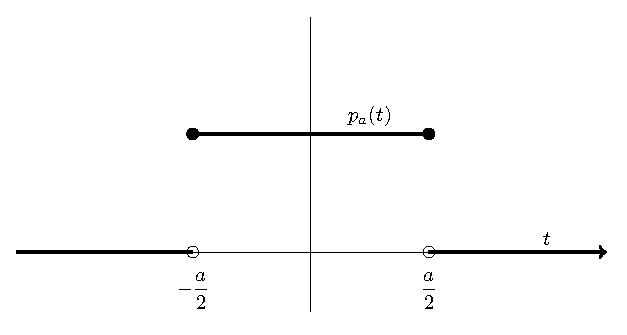
\includegraphics[scale=1]{Imagenes/funcion_paso.eps}
    \caption{Función paso rectangular.}
    \label{fig:figura_funcionpaso}
\end{figure}
Para $\omega \neq 0$ se tiene que la transformada de Fourier es:
\begin{align*}
F \big[p_{a} (\omega)\big] &= \scaleint{6ex}_{\bs -\infty}^{\infty} p_{a}(t) \; \exp{-i \, \omega \, t} \dd{t} = \\[0.5em]
&= \scaleint{6ex}_{\bs -a/2}^{a/2} \exp(-i \, \omega \ t) \dd{t} = \left[ \dfrac{- \exp(- i \, \omega \, t)}{i \, \omega} \right] \eval_{-a/2}^{a/2} \\[0.5em]
&= \dfrac{\exp(i \, a \, \omega/2) - \exp(-i \, a \, \omega/2)}{i \, \omega} = \dfrac{2 \, \sin (a \, \omega/2)}{\omega}
\end{align*}
mientras que para $\omega = 0$, se tiene
\begin{align*}
F \big[p_{a}(0)\big] = \scaleint{6ex}_{\bs -\infty}^{\infty} p_{a}(t) \dd{t} = \scaleint{6ex}_{\bs -a/2}^{a/2} \dd{t} = a
\end{align*}
Es bien sabido que el límite
\begin{align*}
\lim_{x \to 0} \dfrac{\sin x}{x} = 1
\end{align*}
entonces obtenemos 
\begin{align*}
\lim_{\omega \to 0}  (g \, p_{a}) \, (\omega) = \lim_{\omega \to 0} \dfrac{2 \, \sin (a \, \omega /2)}{\omega} = a
\end{align*}
A pesar de que $p_{a}(t)$ en sí, no es continua, vemos que
\begin{align}
F \big[p_{a}(\omega)\big] = \dfrac{2 \sin (a \, \omega/2)}{\omega}
\label{eq:ecuacion_06_11_Beerends}
\end{align}
es continua en $\mathbb{R}$.
\begin{figure}[H]
    \centering
    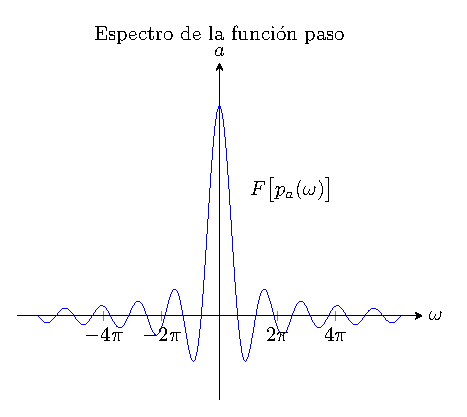
\includegraphics[scale=1.3]{Imagenes/T_Funcionpaso.eps}
    \caption{Transformada de Fourier de la función paso rectangular.}
    \label{fig:figura_Tfuncionpaso}
\end{figure}
% \textbf{Problema a cuenta: } Calcula la transformada de Fourier de un pulso triangular, como se muestra en la siguiente figura:
% \begin{figure}[H]
%     \centering
%     \includestandalone{Figuras/Tarea-01-Pulso_Triangular}
% \end{figure}
% \begin{align*}
% f (x) = \begin{cases}
% h(1 - a \, \abs{x}) & \abs{x} < \dfrac{1}{a} \\
% 0 & \abs{x} > \dfrac{1}{a}
% \end{cases}
% \end{align*}

\subsection*{Ejemplo 8.}

La ecuación de calor: la temperatura $u (x, t)$ de una barra semiinfinita está determinada por la EDP:
\begin{align*}
\pdv{u}{t} = \pdv[2]{u}{x} \hspace{1.5cm} x > 0, t > 0
\end{align*}
sujeta a la condición inicial:
\begin{align*}
u (x, 0) = \begin{cases}
1, & 0 < x < 1  \\
0, & x > 1
\end{cases}
\end{align*}
y la condición de frontera $u (0, t) = 0$, ver la figura (\ref{fig:figura_plot_Ejemplo_06_01}). Determina la temperatura en la barra para cualquier tiempo $t$ y en cualquier distancia $x$ a partir de $x = 0$.
\begin{figure}[H]
    \centering
    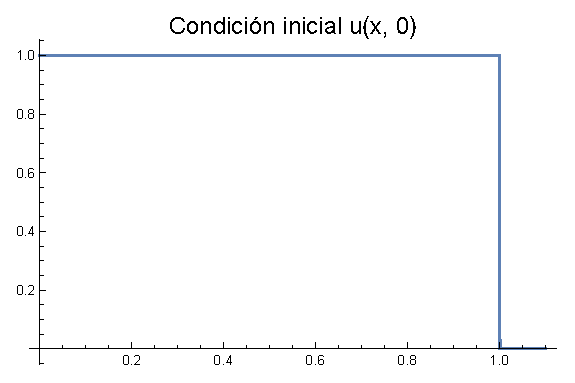
\includegraphics[scale=1]{Imagenes/Plot_Ejemplo_06_01.eps}
    \caption{Estado inicial de la barra.}
    \label{fig:figura_plot_Ejemplo_06_01}
\end{figure}

\noindent
\textbf{Solución: } Dado que la variable $x$ cambia de $0$ a $\infty$ y como el valor de $u(x, t)$ en $x = 0$ está indicado, podemos tomar la transformada seno de Fourier en ambos lados de la EDP para la variable $x$, que queda excluida de la ecuación transformada. Se tiene entonces que la ecuación dada es:
\begin{align*}
\dv{t} \overline{u}_{s} (\xi, t) &= \sqrt{\dfrac{2}{\pi}} \scaleint{6ex}_{\bs 0}^{\infty} \pdv[2]{u}{x} \sin \xi x \dd{x} = \\[0.5em]
&= \sqrt{\dfrac{2}{\pi}} \, \big[ \xi \, u(0, t) \big] - \xi^{2} \, \overline{u}_{s} (\xi, t) = \\[0.5em]
&= - \xi^{2} \, \overline{u}_{s} (x , t)
\end{align*}
por lo que:
\begin{align}
\overline{u}_{s} (\xi, t) = c \, \exp(-\xi^{2} \, t)
\label{eq:ecuacion_ejemplo_1_27_i}
\end{align}
donde $c$ es una constante arbitraria.
\par
Como se tiene la condición inicial:
\begin{align}
\begin{aligned}
u (x, 0) &= \begin{cases}
1, & 0 < x < 1  \\
0, & x > 1
\end{cases}
\\
\therefore \quad \overline{s}_{s} (\xi, 0) &= \sqrt{\dfrac{2}{\pi}} \scaleint{6ex}_{\bs 0}^{\infty} u (x, 0) \sin \xi x \dd{x} \\[0.5em]
&= \sqrt{\dfrac{2}{\pi}} \scaleint{6ex}_{\bs 0}^{1} \sin \xi x \dd{x} = \\[0.5em]
&= \sqrt{\dfrac{2}{\pi}} \, \bigg[ \dfrac{- \cos \xi x}{\xi} \bigg] \eval_{0}^{1} = \\[0.5em]
&= \sqrt{\dfrac{2}{\pi}} \, \bigg[ \dfrac{1 - \cos \xi}{\xi} \bigg]
\end{aligned}
\label{eq:ecuacion_ejemplo_1_27_ii}
\end{align}
Por lo que, de las ecs. (\ref{eq:ecuacion_ejemplo_1_27_i}) y (\ref{eq:ecuacion_ejemplo_1_27_ii}), tenemos que:
\begin{align*}
c = \sqrt{\dfrac{2}{\pi}} \, \bigg[ \dfrac{1 - \cos \xi}{\xi} \bigg]
\end{align*}
Ocupando este valor de $c$ en la ec. (\ref{eq:ecuacion_ejemplo_1_27_i}), se llega a:
\begin{align*}
u (x, t) = \dfrac{2}{\pi} \scaleint{6ex}_{\bs 0}^{\infty} \dfrac{1 - \cos \xi}{\xi} \, \exp(-\xi^{2} t) \, \sin \xi x\dd{\xi}
\end{align*}
Que es la función de temperatura $u (x, t)$ que se pidió en el inciso del ejercicio y que se muestra en la figura (\ref{fig:figura_plot_Ejemplo_06_02}), al tener dos variables $x$, $t$, la gráfica resulta una superficie.
\begin{figure}[H]
    \centering
    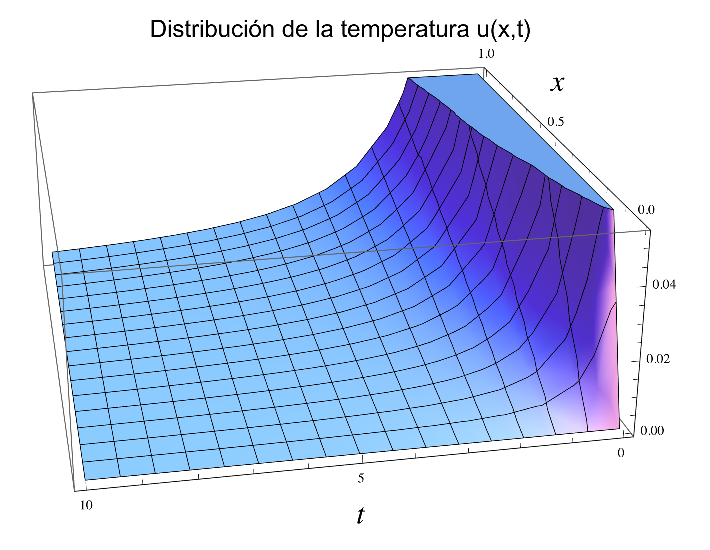
\includegraphics[scale=1]{Imagenes/Plot_Ejemplo_06_02.eps}
    \caption{Distribución de temperaturas en la barra como función de la posición $x$ y del tiempo $t$.}
    \label{fig:figura_plot_Ejemplo_06_02}
\end{figure}

\subsection*{Ejemplo 9.}

La ecuación de onda: Con la transformada de Fourier determina el desplazamiento $y(x, t)$ en una cuerda infinita oscilante, considerando que la cuerda está inicialmente en reposo y que el desplazamiento inicial es $f (x)$ para $-\infty < x < \infty$. Demuestra que la solución se presenta de la forma:
\begin{align*}
y(x, t) = \dfrac{1}{2} \big[ f(x + c \, t) + f(x - c \, t) \big]
\end{align*}
\par
\noindent
\textbf{Solución: } La ecuación de onda unidimensional de una cuerda oscilante está dada por:
\begin{align*}
\pdv[2]{y}{t} = c^{2} \pdv[2]{y}{x}, \hspace{1.5cm} -\infty < x < \infty, \hspace{0.2cm} t > 0
\end{align*}

Ya que la variable $x$ cambia de $-\infty$ a $\infty$, para remover la variable de la EDP, ocupamos la transformada de Fourier compleja en la ecuación de onda para obtener:
\begin{align*}
\dv[2]{\overline{y}(\xi, t)}{t} &= \dfrac{c^{2}}{\sqrt{2 \pi}} \scaleint{6ex}_{\bs -\infty}^{\infty} \pdv[2]{y(x, t)}{x} \, \exp(i \xi x) \dd{x} = \\[0.5em]
&= - c^{2} \, \xi^{2} \, \overline{y} (\xi, t)
\end{align*}
Por lo tanto:
\begin{align}
\overline{y} (\xi, t) &= A \, \cos (c \, \xi \, t) + B \, \sin (c \, \xi \, t) \label{eq:ecuacion_ejemplo_1_29_i} \\[0.5em]
\overline{y}_{t} (\xi, t) &= A \, c \, \xi \, \sin (c \, \xi \, t) + B \, c \, \xi \, \cos (c \, \xi \, t) \label{eq:ecuacion_ejemplo_1_29_ii}
\end{align}
donde $A$ y $B$ son dos constantes arbitrarias. Ahora, las condiciones iniciales son:
\begin{align}
y(x, 0) &= \mbox{desplazamiento inicial } = f (x) \label{eq:ecuacion_ejemplo_1_29_iii} \\[0.5em]
\pdv{y}{t} (x, 0) &= 0 \hspace{0.5cm} \mbox{ya que la velocidad inicial de la cuerda es cero} \label{eq:ecuacion_ejemplo_1_29_iv}
\end{align}
De las ecs. (\ref{eq:ecuacion_ejemplo_1_29_ii}) y (\ref{eq:ecuacion_ejemplo_1_29_iii}), se tiene que:
\begin{align}
\overline{y} (\xi, t) &= \dfrac{1}{\sqrt{2 \pi}} \scaleint{6ex}_{\bs -\infty}^{\infty} f (x) \, \exp(i \xi x) \dd{x} = \overline{f} (\xi) \label{eq:ecuacion_ejemplo_1_29_v} \\[0.5em]
\pdv{\overline{y}}{t} (\xi, 0) &= \overline{y}_{t} (\xi, 0) = 0 \label{eq:ecuacion_ejemplo_1_29_vi}
\end{align}
De la ec. (\ref{eq:ecuacion_ejemplo_1_29_i}), se tiene que:
\begin{align}
\overline{y} (\xi, 0) = A = \overline{f} (\xi) \hspace{1.5cm} \mbox{por la ec. (\ref{eq:ecuacion_ejemplo_1_29_v})}
\end{align}
También por la ec. (\ref{eq:ecuacion_ejemplo_1_29_ii}), se obtiene:
\begin{align}
\overline{y}_{t} (\xi, 0) = B \, c \, \xi \hspace{1.5cm} \mbox{por la ec. (\ref{eq:ecuacion_ejemplo_1_29_vi})}
\end{align}
Entonces  $B = 0$. Así:
\begin{align*}
\overline{y}(\xi, t) = \overline{f}(\xi) \, \cos (c \, \xi \, t)
\end{align*}
Tomando la transformada inversa de la ecuación anterior, se llega a:
\begin{align*}
y(x, t) &= \dfrac{1}{\sqrt{2 \pi}} \scaleint{6ex}_{\bs \infty}^{+ \infty} \bigg[ \dfrac{\exp(i c \xi t) + \exp(-i c \xi t)}{2} \bigg] \, \exp(-i \, \xi \, x) \dd{\xi} = \\[0.5em]
&= \dfrac{1}{2} \, \dfrac{1}{\sqrt{2 \pi}} \scaleint{6ex}_{\bs \infty}^{+ \infty} \overline{f} (\xi) \cdot \bigg[ \exp(-i \xi (x {-} c t)) {+} \exp(-i \xi (x {+} c t)) \bigg] \dd{\xi} = \\[0.5em]
&= \dfrac{1}{2} \bigg[ \dfrac{1}{\sqrt{2 \pi}} \scaleint{6ex}_{-\infty}^{+\infty} \overline{f} (\xi) \, \exp(- \xi (x - c t)) \dd{\xi} + \\[0.5em]
&+ \dfrac{1}{2} \dfrac{1}{\sqrt{2 \pi}} \scaleint{6ex}_{-\infty}^{+\infty} \overline{f} (\xi) \cdot \exp(- \xi (x + c t)) \dd{\xi} \bigg] \\[0.5em]
\Rightarrow \hspace{0.3cm} y(x, t) &= \dfrac{1}{2} \big[ f(x -c t) + f(x +  ct) \big]
\end{align*}

% \newpage
% \section{Ejercicios a cuenta.}

% \noindent
% %Ref. Patra Example 1.5
% \textbf{Ejercicio a cuenta (57). } Calcula la transformada de Fourier de:
% \begin{align*}
% f (x) = \begin{cases}
% 1 - x^{2}, & \abs{x} \leq 1 \\
% 0, & \abs{x} > 1
% \end{cases}
% \end{align*}
% y con ese resultado, evalúa la siguiente integral:
% \begin{align*}
% \scaleint{6ex}_{\bs0}^{\infty} \dfrac{x \, \cos x - \sin x}{x^{3}} \, \cos \dfrac{x}{2} \dd{x}
% \end{align*}

% \noindent
% %Ref. Patra Example 1.12
% \textbf{Ejercicio a cuenta (58). } Con las siguientes funciones:
% \begin{align*}
% g(x) = e^{-a x} \hspace{2cm} f (x) \begin{cases}
% 1, & 0 < x < b \\
% 0, & x > b
% \end{cases} 
% \end{align*}
% y con la relación de Parseval pertinente, demuestra que:
% \begin{align*}
% \scaleint{6ex}_{\bs 0}^{\infty} \dfrac{\sin a t}{t (a^{2} + t^{2})} \dd{t} = \dfrac{\pi}{2} \, \dfrac{1 - \exp(-a^{2})}{a^{2}}
% \end{align*}
% \\[0.5em]
% \noindent
% %Ref. Patra Example 1.38
% \textbf{Ejercicio a cuenta (59). } La temperatura $u(x, t)$ en una barra semiinfinita $0 \leq x < \infty$ satisface la siguiente EDP:
% \begin{align*}
% \pdv{u}{t} =\kappa \, \pdv[2]{u}{x}
% \end{align*}
% sujeta a las siguientes condiciones:
% \begin{align*}
% u(x, 0) &= 0, \hspace{0.5cm} x \geq 0 \\[0.5em]
% \pdv{u}{x} &= - \lambda \hspace{0.5cm} \mbox{una constante, cuando \quad} x = 0, \hspace{0.2cm} t > 0  
% \end{align*}
% Calcula la temperatura para valores $x > 0$ y $t > 0$.
\end{document}